% Digital Logic Lab 10 7-Segment Display with Time-Division Multiplexing
% Created: 2020-05-01, Megan Gordon

%==========================================================
%=========== Document Setup  ==============================

% Formatting defined by class file
\documentclass[11pt]{article}

% ---- Document formatting ----
\usepackage[margin=1in]{geometry}	% Narrower margins
\usepackage{booktabs}				% Nice formatting of tables
\usepackage{graphicx}				% Ability to include graphics

%\setlength\parindent{0pt}	% Do not indent first line of paragraphs 
\usepackage[parfill]{parskip}		% Line space b/w paragraphs
%	parfill option prevents last line of pgrph from being fully justified

% Parskip package adds too much space around titles, fix with this
\RequirePackage{titlesec}
\titlespacing\section{0pt}{8pt plus 4pt minus 2pt}{3pt plus 2pt minus 2pt}
\titlespacing\subsection{0pt}{4pt plus 4pt minus 2pt}{-2pt plus 2pt minus 2pt}
\titlespacing\subsubsection{0pt}{2pt plus 4pt minus 2pt}{-6pt plus 2pt minus 2pt}

% ---- Hyperlinks ----
\usepackage[colorlinks=true,urlcolor=blue]{hyperref}	% For URL's. Automatically links internal references.

% ---- Code listings ----
\usepackage{listings} 					% Nice code layout and inclusion
\usepackage[usenames,dvipsnames]{xcolor}	% Colors (needs to be defined before using colors)

% Define custom colors for listings
\definecolor{listinggray}{gray}{0.98}		% Listings background color
\definecolor{rulegray}{gray}{0.7}			% Listings rule/frame color

% Style for Verilog
\lstdefinestyle{Verilog}{
	language=Verilog,					% Verilog
	backgroundcolor=\color{listinggray},	% light gray background
	rulecolor=\color{blue}, 			% blue frame lines
	frame=tb,							% lines above & below
	linewidth=\columnwidth, 			% set line width
	basicstyle=\small\ttfamily,	% basic font style that is used for the code	
	breaklines=true, 					% allow breaking across columns/pages
	tabsize=3,							% set tab size
	commentstyle=\color{gray},	% comments in italic 
	stringstyle=\upshape,				% strings are printed in normal font
	showspaces=false,					% don't underscore spaces
}

% How to use: \Verilog[listing_options]{file}
\newcommand{\Verilog}[2][]{%
	\lstinputlisting[style=Verilog,#1]{#2}
}




%======================================================
%=========== Body  ====================================
\begin{document}

\title{ELC 2137 Lab 11: FSM: Guessing Game}
\author{Megan Gordon}

\maketitle


\section*{Summary}

This lab looks to expand on previous labs by expanding into larger systems with more modules. It allowed us to learn how to explain the role of finite state machines in digital systems logic, explain the difference between a Mealy output and a Moore output, and implement a state machine in Verilog. In completing this lab, the following skills were gained: ability to recognize and run a debounce circuit, the ability to develop a game using Mealy or Moore outputs, the ability to implement a clock-driven, guessing game using pushbuttons, leds, switches, and an instance of a counter module. 



\section*{Results}

\textbf{Deliverable Questions:}

\medskip
\textbf{a)} At what time in the simulation did the debounce circuit reach each of the four states? (zero, wait1, one, wait0)?
\textbf	The debounce circuit reaches each of the for states at around the following times: zero at 20ns, wait1 at 200ns, one at 245ns, and wait0 at 420ns. 

\textbf{b)} Why can this game not be implemented with regular sequential logic?
\textbf	If implemented with regular sequential logic, the game would not skip to win or skip to lose without going through the entire states of s0, s1, s2, and s3. 


\textbf{c)} What type of outputs did you use for your design (Mealy or Moore)? 
\textbf	I used Moore outputs for my design. Although it can be slower to operate, it has less probability of total failure.
\clearpage

\textbf{Below are the simulations for the modules, debounce and guess FSM and pictures of the board for win and lose for on-board testing of guessing game.} 
\bigskip
\bigskip
\bigskip

\begin{figure}[ht]\centering
	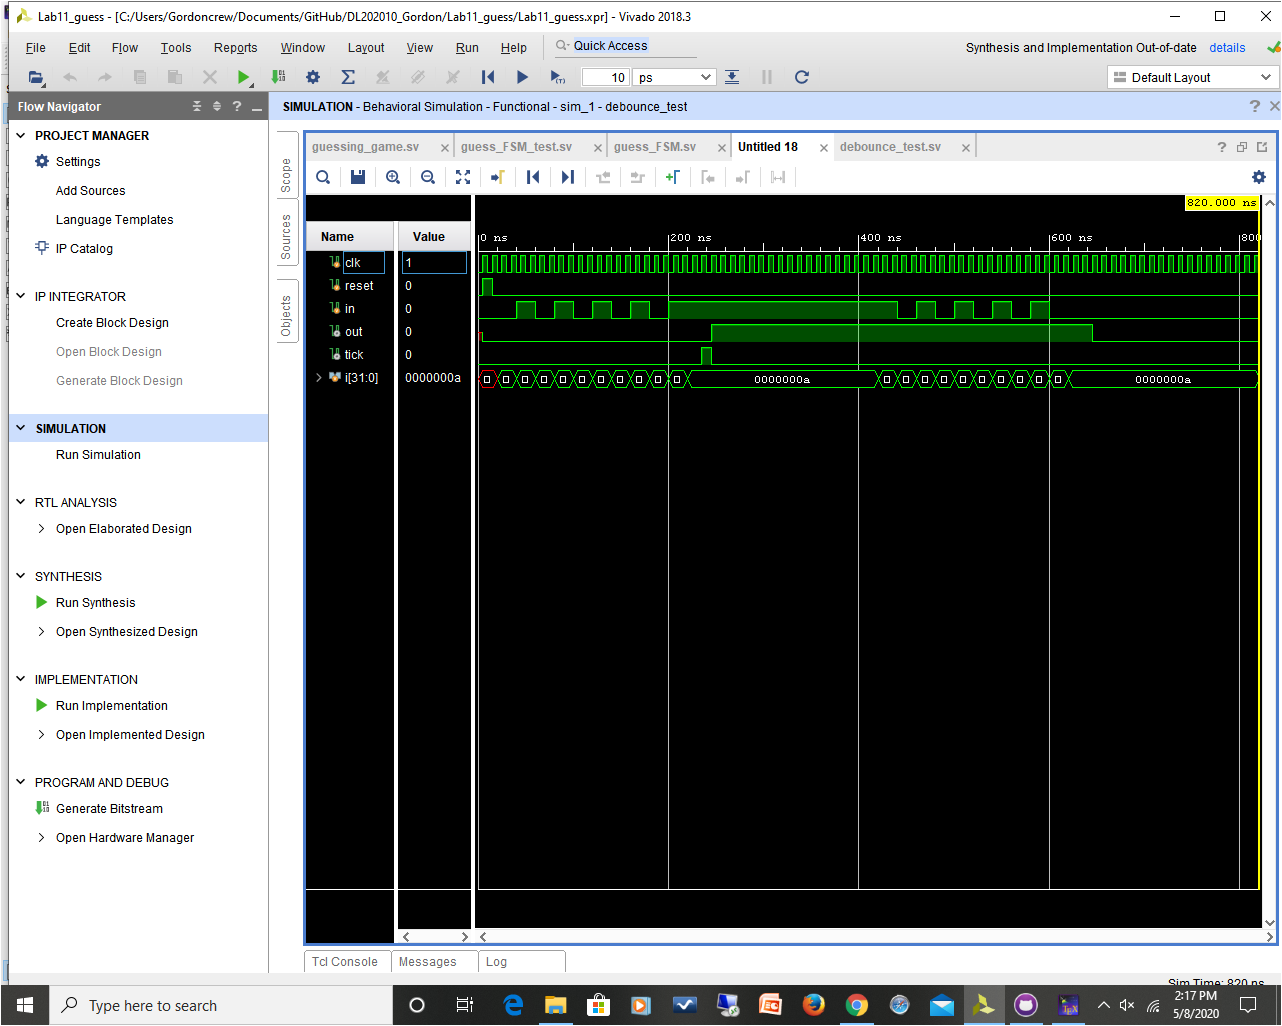
\includegraphics[width=1.15\textwidth, trim=7.5cm 14cm 0cm 4cm,clip]{debounce.png}
	\caption{Debounce Simulation Results}
	\label{fig:sim_with_table}
\end{figure}


\begin{figure}[ht]\centering
	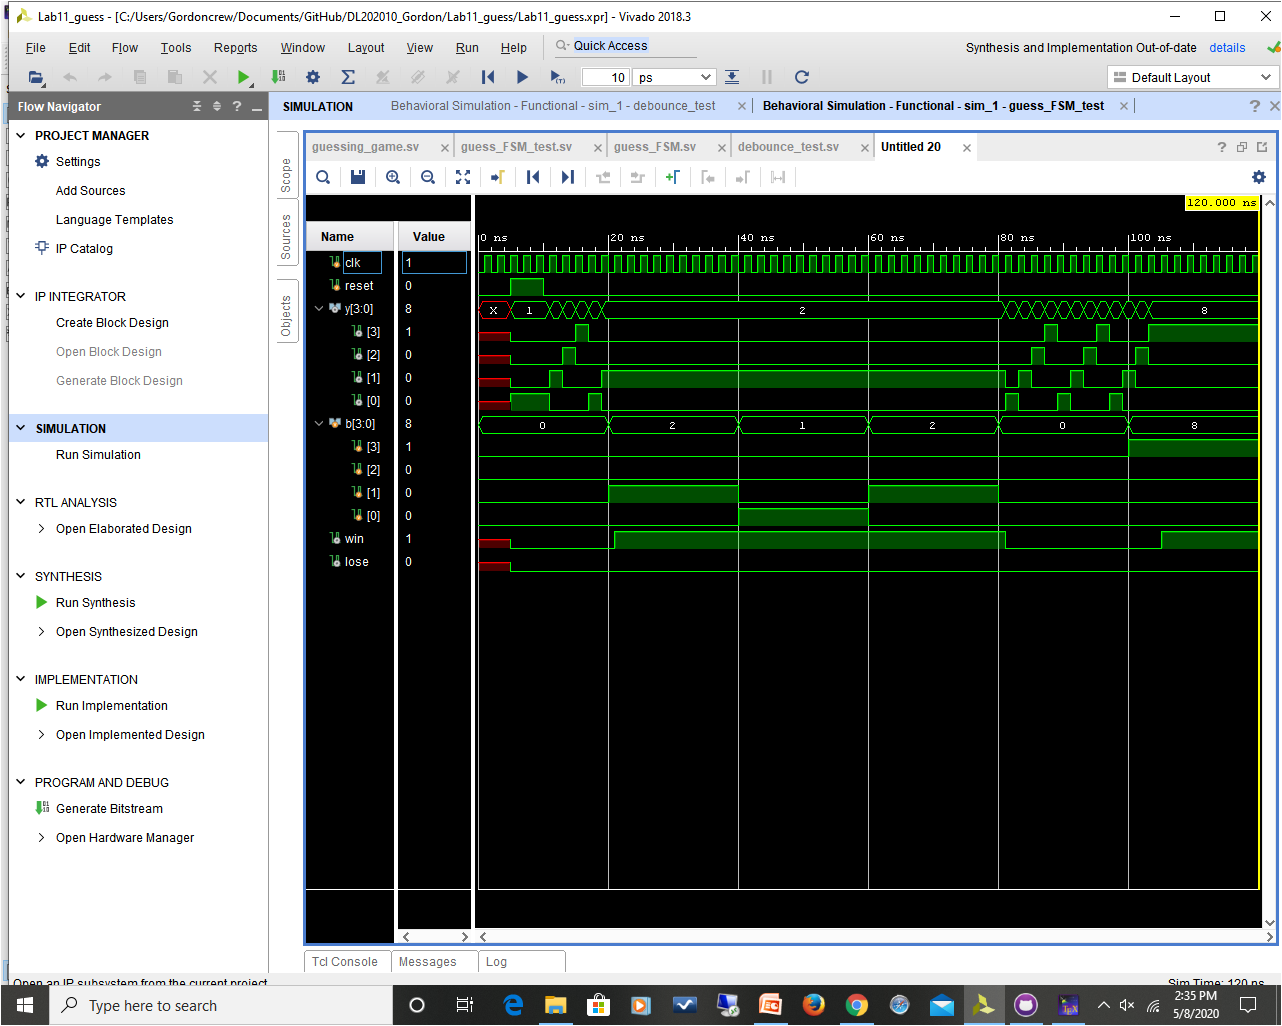
\includegraphics[width=1.15\textwidth, trim=7.5cm 10cm 0cm 4.0cm,clip]{guess_FSM.png}
	\caption{Guess FSM Simulation Results}
	\label{fig:sim_with_table}
\end{figure}


\clearpage

\begin{figure}[ht]\centering
	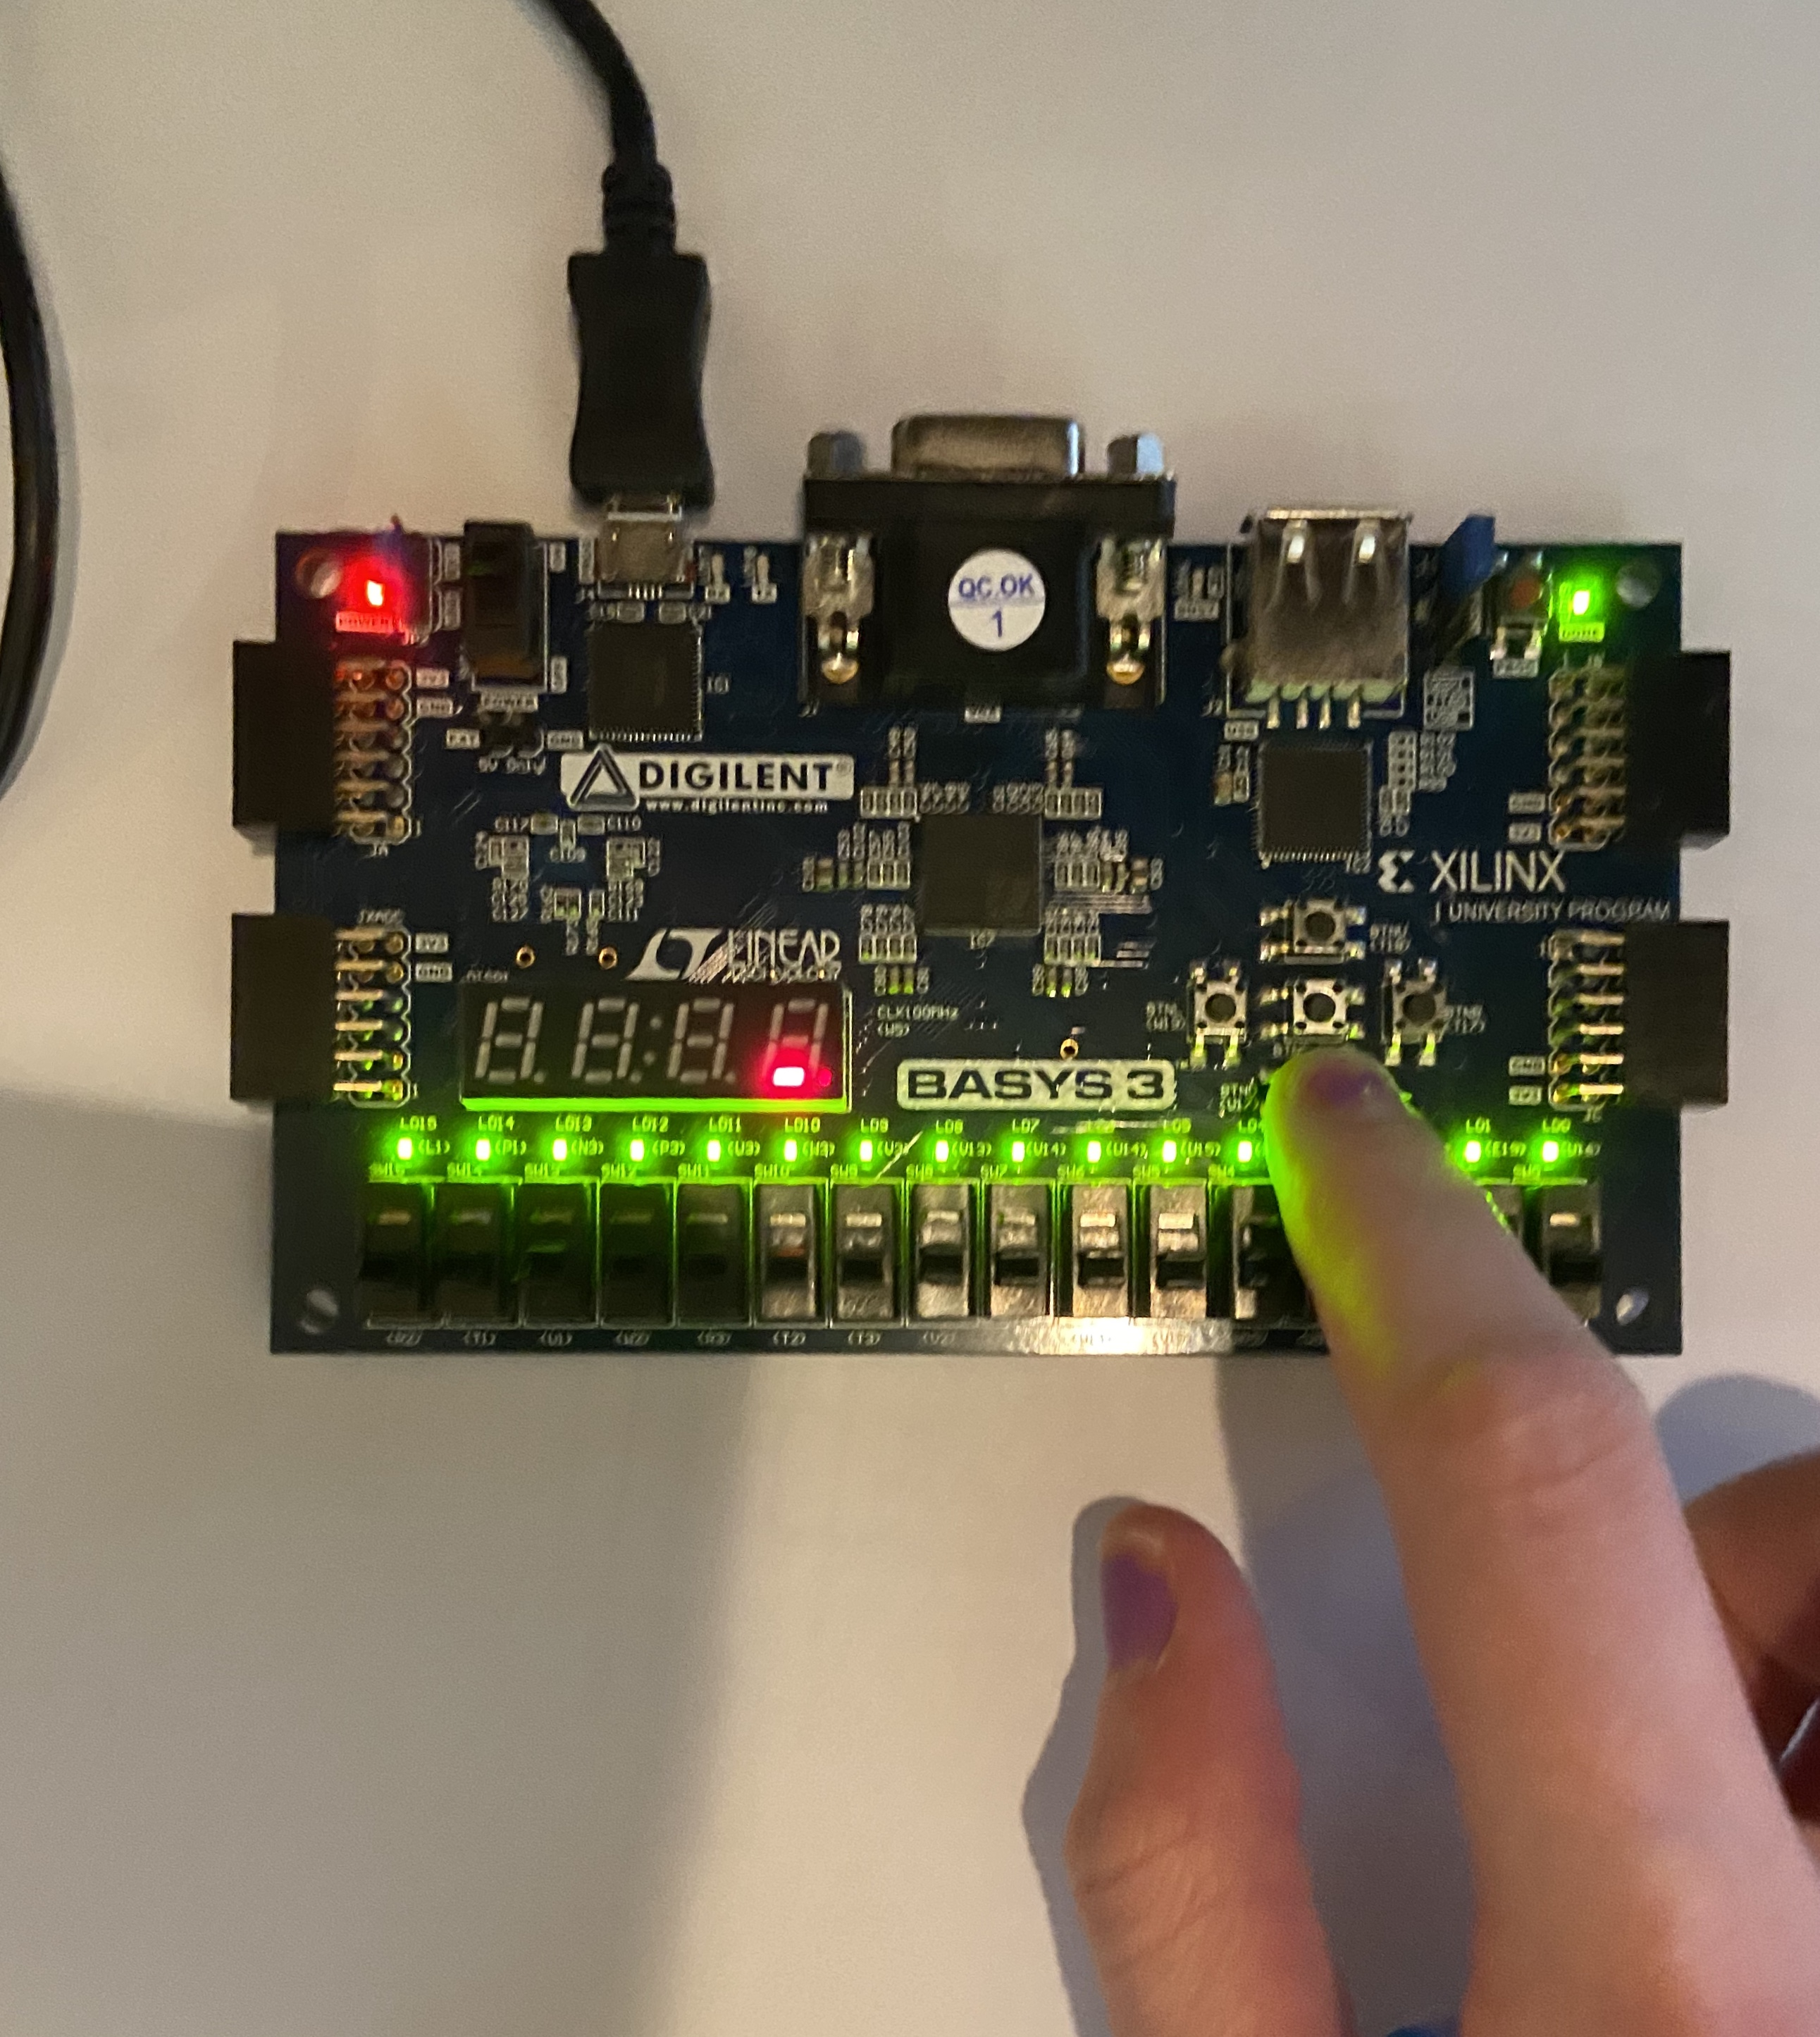
\includegraphics[angle=0, width=1.0\textwidth]{IMG_7264.jpg}
	\caption{Game Results Simulation 1 - Win}
	\label{fig:sim_with_table}
\end{figure}
\clearpage

\begin{figure}[ht]\centering
	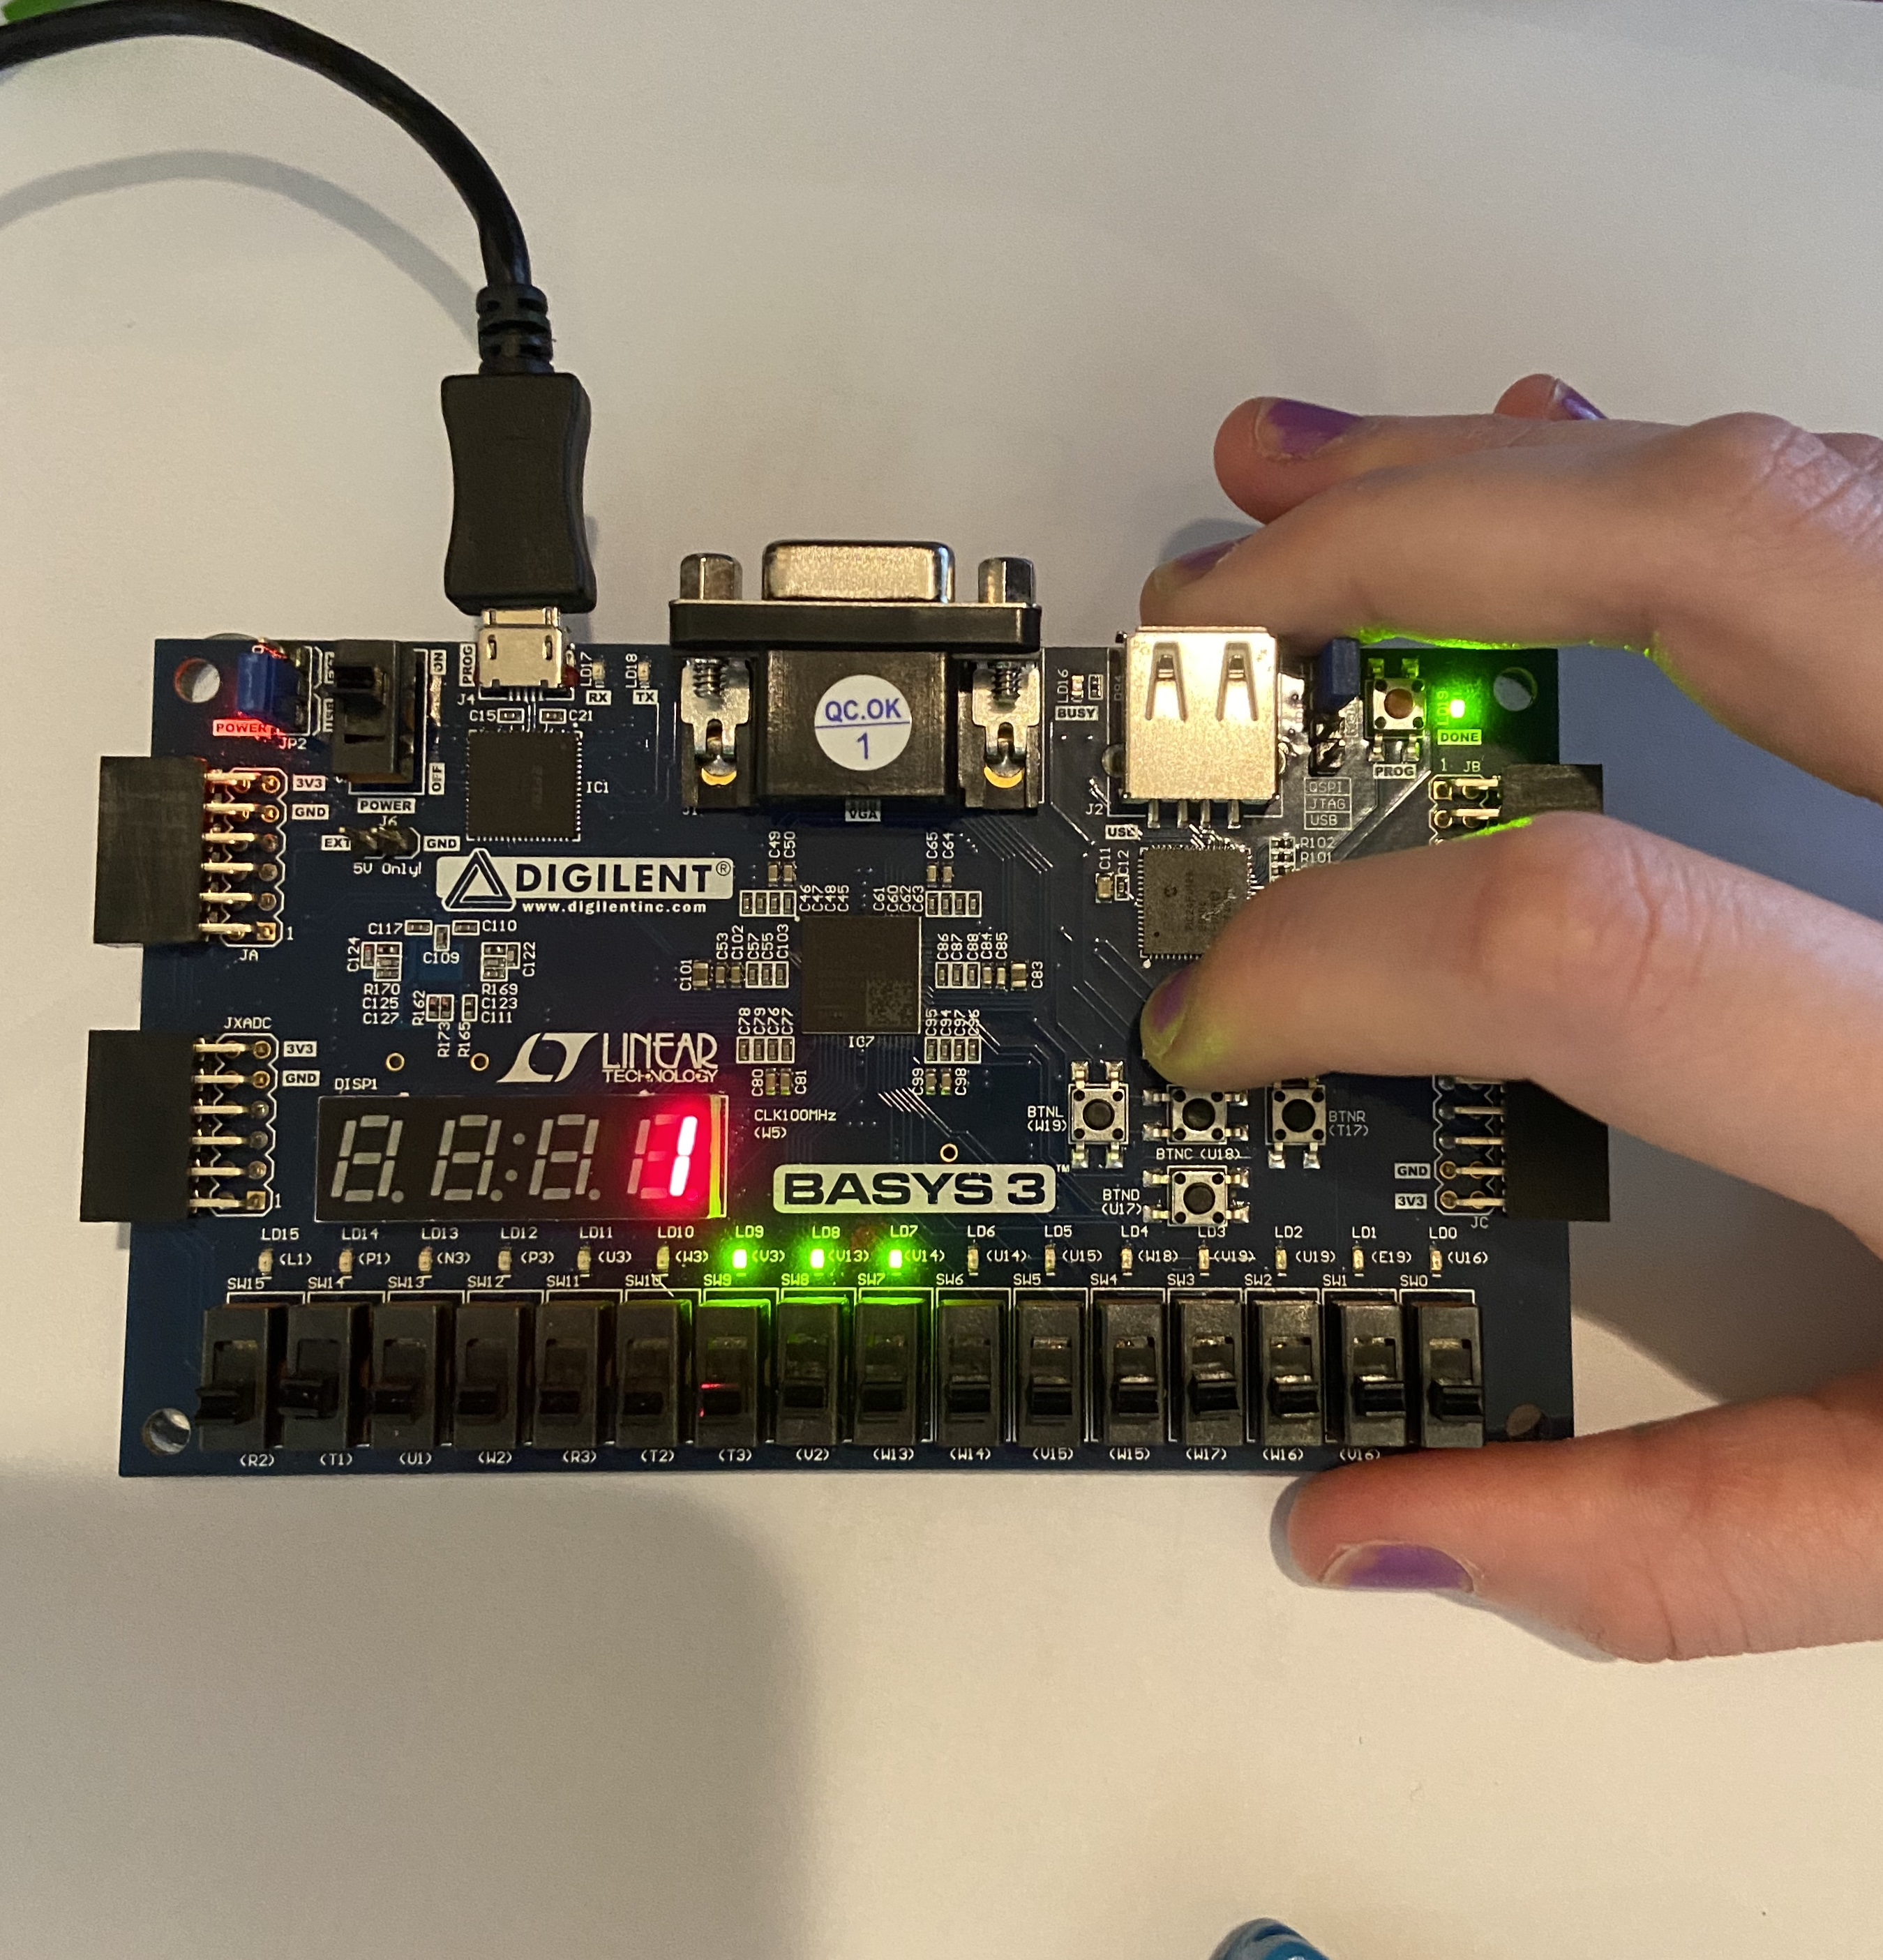
\includegraphics[angle=0, width=1.0\textwidth]{IMG_7266.jpg}
	\caption{Game Results Simulation 2 - Lose}
	\label{fig:sim_with_table}
\end{figure}
\clearpage

\begin{figure}[ht]\centering
	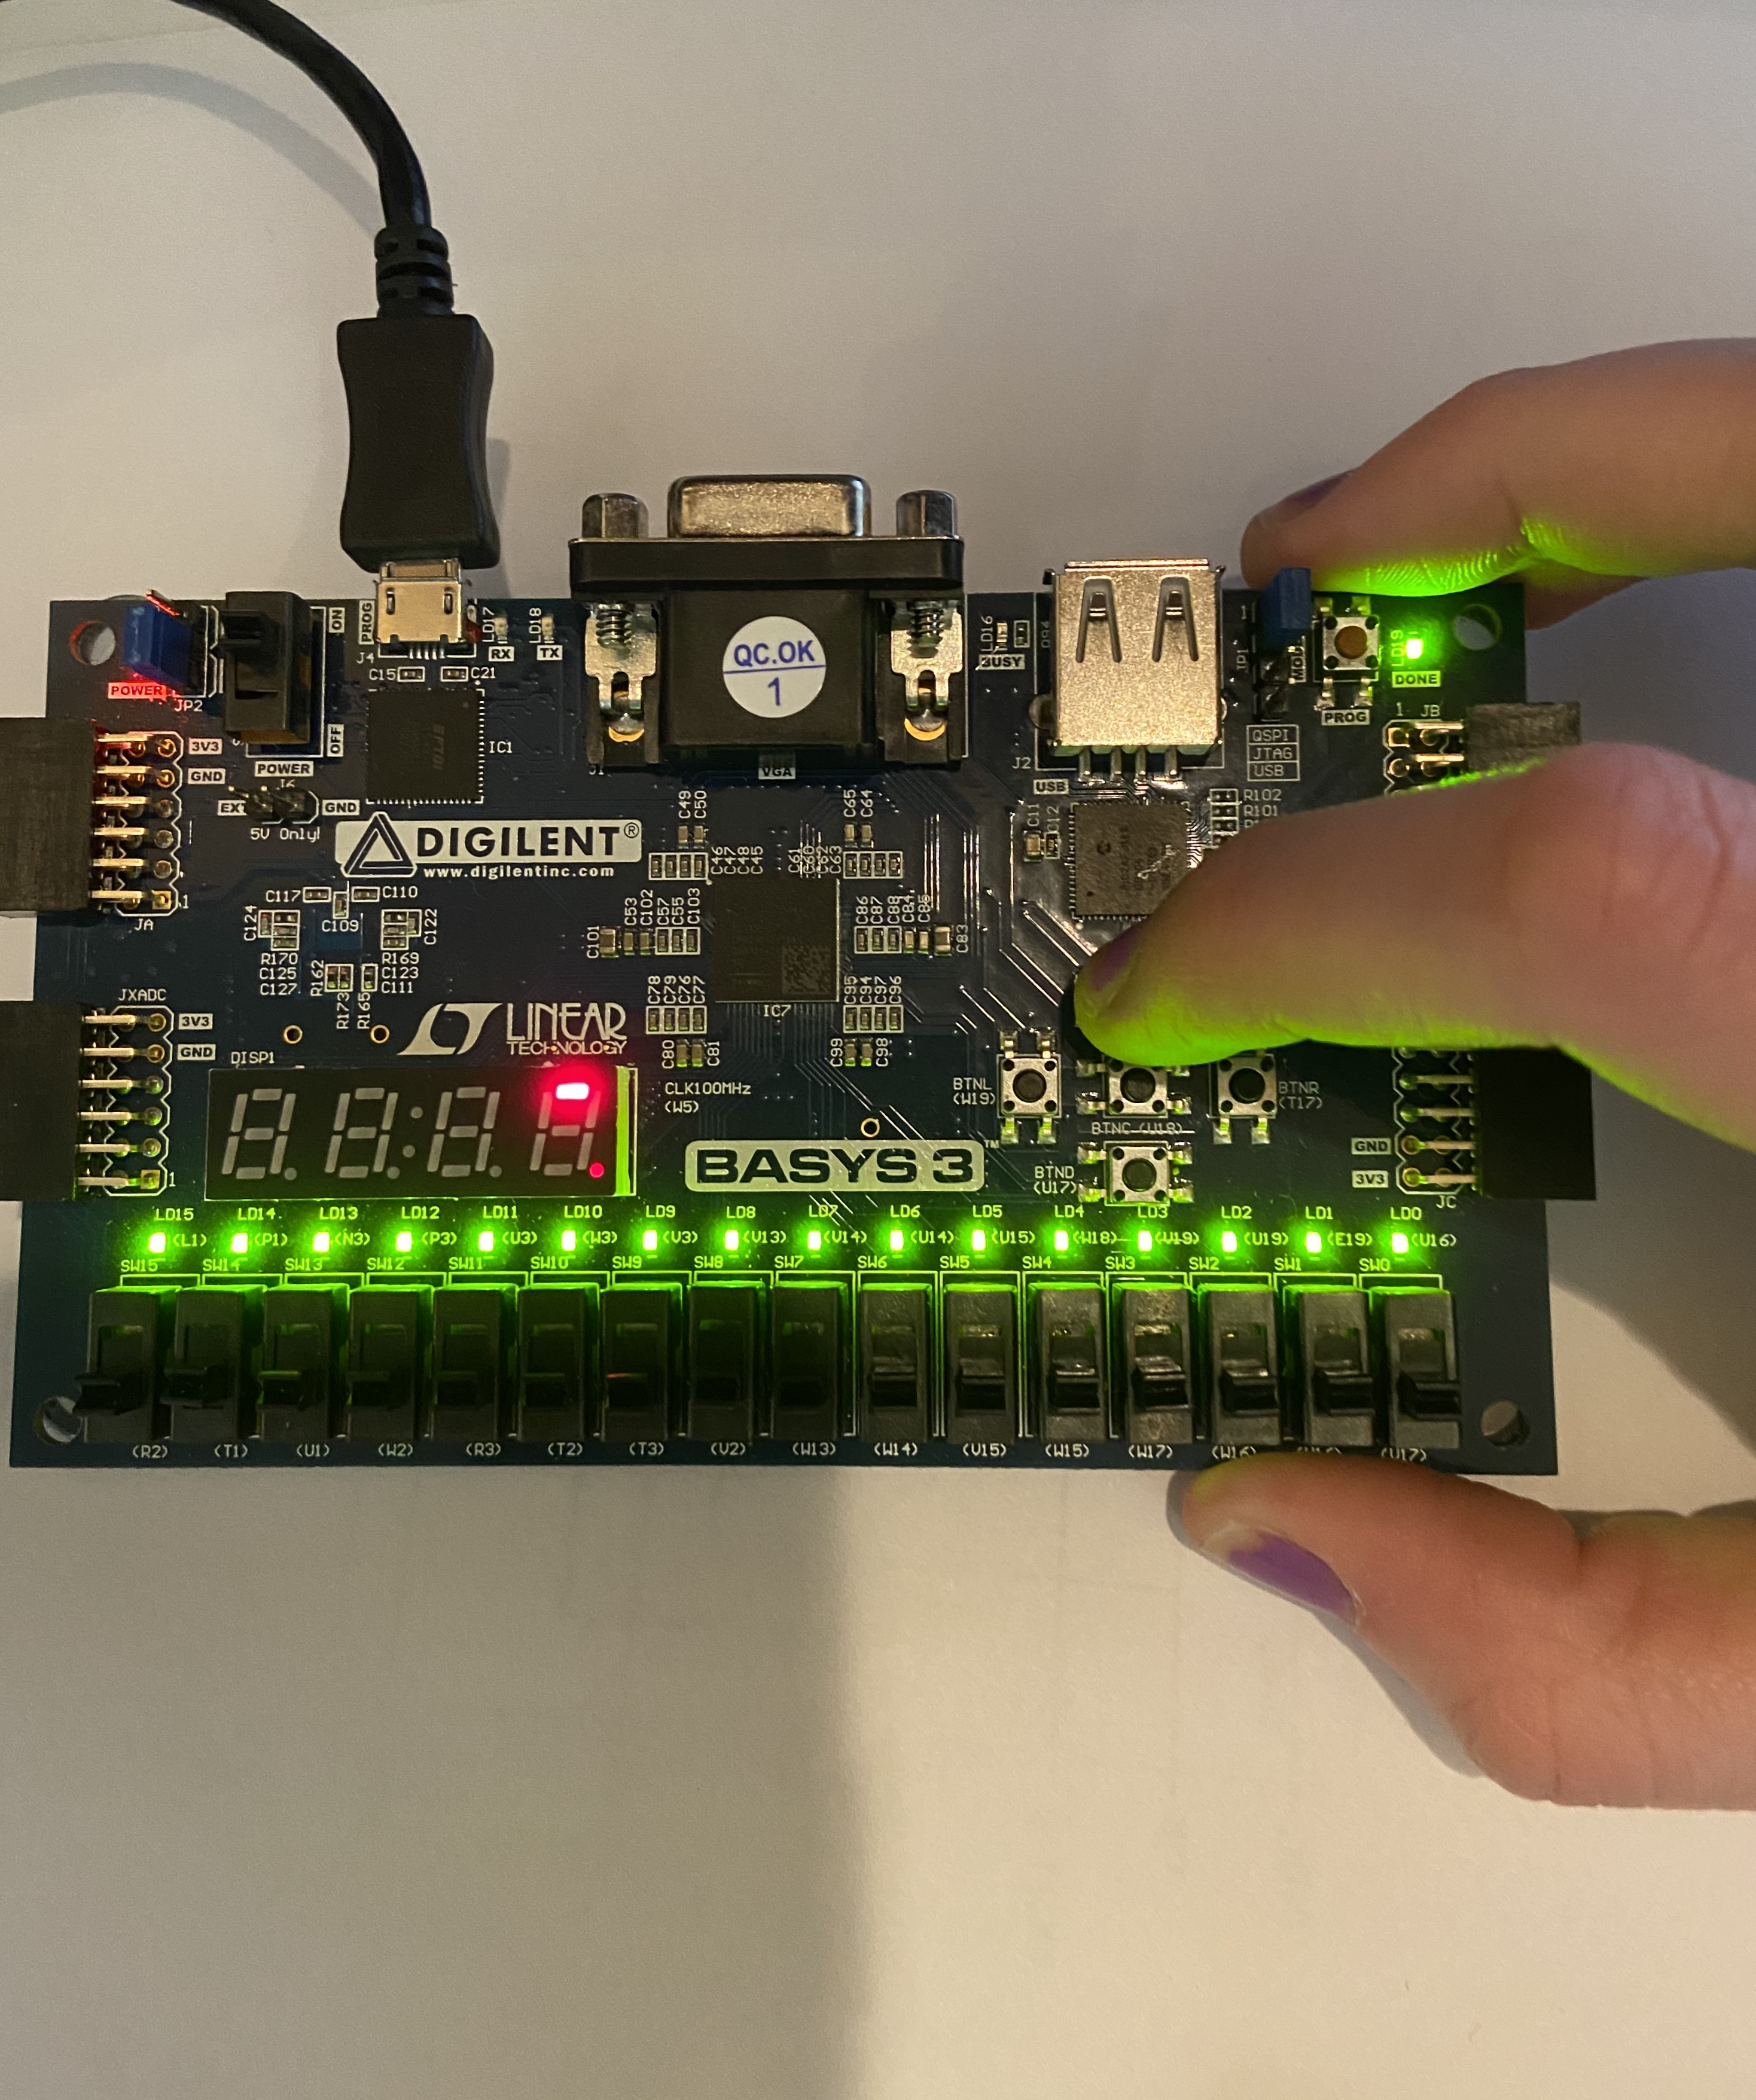
\includegraphics[angle=0, width=1.0\textwidth]{IMG_7265.jpg}
	\caption{Game Results Simulation 3 - Win}
	\label{fig:sim_with_table}
\end{figure}
\clearpage

\begin{figure}[ht]\centering
	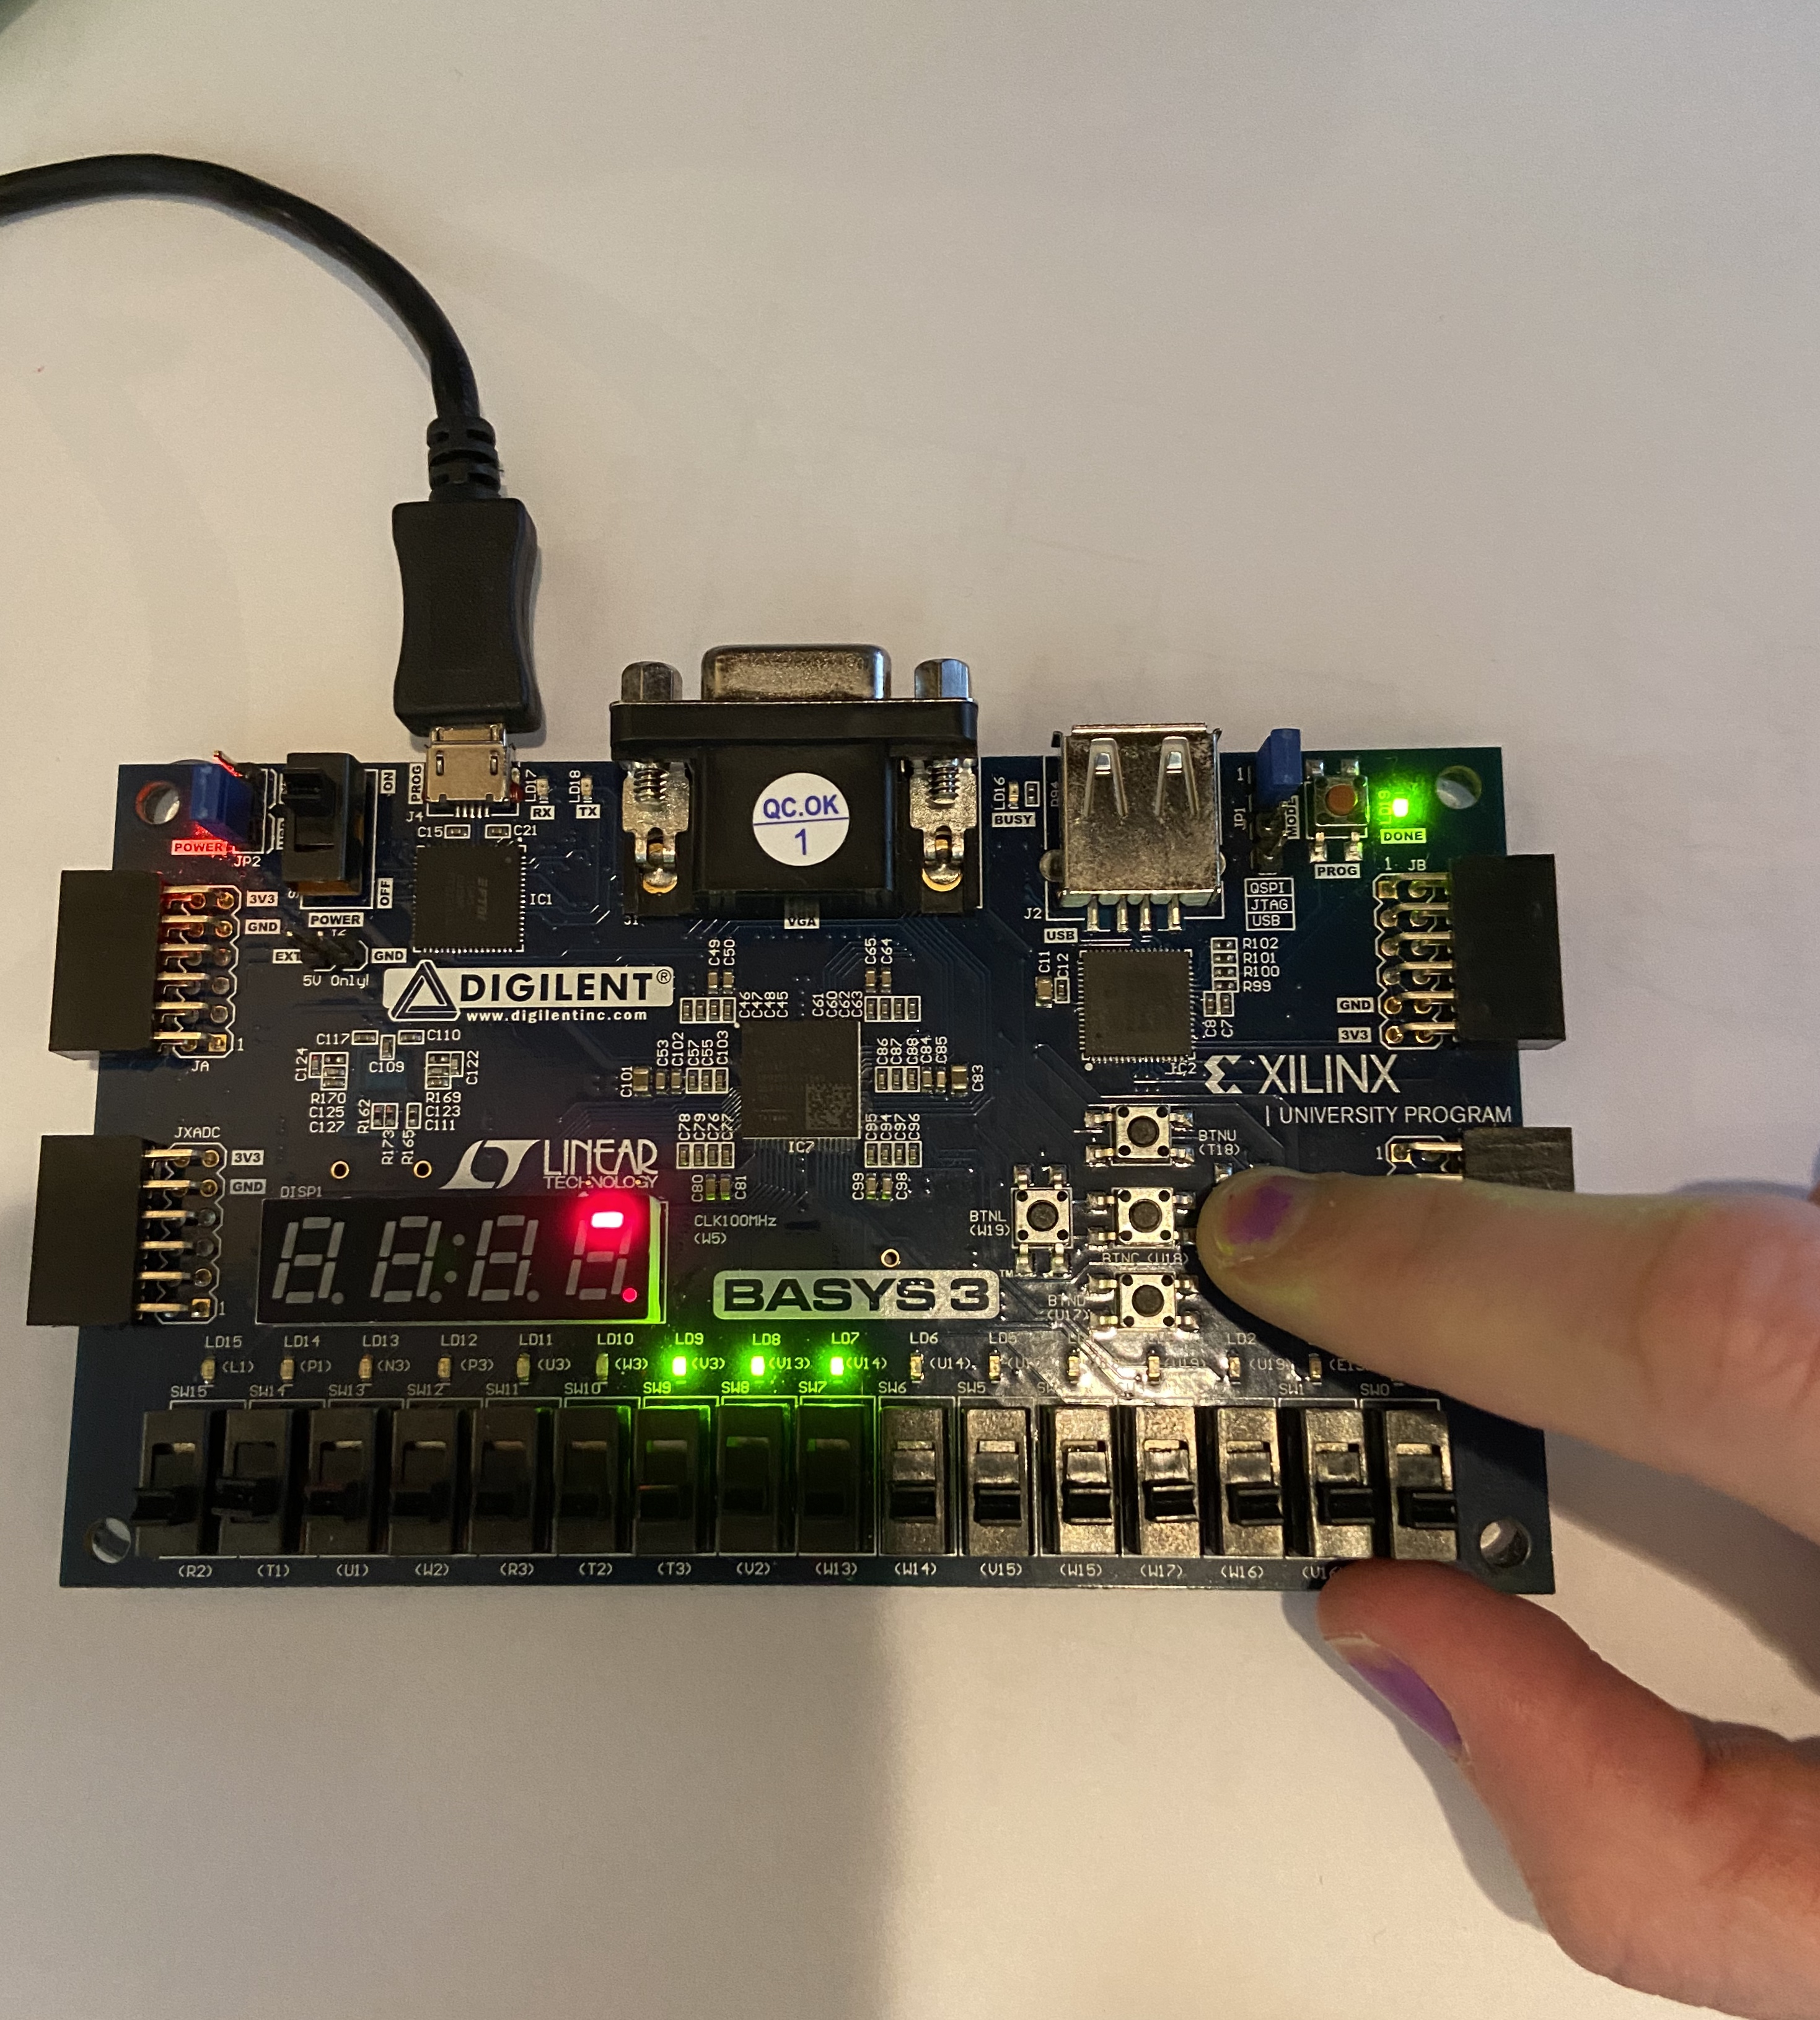
\includegraphics[angle=0, width=1.0\textwidth]{IMG_7267.jpg}
	\caption{Game Results Simulation 4 - Lose}
	\label{fig:sim_with_table}
\end{figure}
\clearpage



\section*{Code}

Code for source files for debounce, guess FSM, and guessing game and the test bench files for the debounce and guess FSM.

\begin{lstlisting}[style=Verilog,caption=debounce Code,label=code:ex ]

`timescale 1ns / 1ps
// ELC 2137, John Miller, 2019-11-08 

module debounce #(parameter N=21)
(input clk, reset,
input  in,
output reg out,
output reg tick);

// define states as local parameters (constants)
localparam [1:0]
zero   = 2'b00,
wait1  = 2'b01,
one    = 2'b11,
wait0  = 2'b10;

// internal signals
reg [1:0] state, state_next;
reg [N-1:0] counter, counter_next;

// state memory (register)
always_ff @(posedge clk or posedge reset)
if (reset) begin
state   <= zero;
counter <= {N{1'b1}};
end
else begin
state   <= state_next;
counter <= counter_next;
end

// combined next-state and output logic
always_comb begin
// default behavior
state_next   = state;
counter_next = counter;
tick = 0;

case(state)
zero: begin
out = 0;
counter_next = {N{1'b1}};
if (in)
state_next = wait1;
end

wait1: begin
out = 0;     // Moore output
counter_next = counter - 1;
if (counter == 0) begin
tick = 1'b1; // Mealy output
state_next = one;
end
else if (~in)
state_next = zero;
end

one: begin
out = 1;
counter_next = {N{1'b1}};
if (~in)
state_next   = wait0;
end

wait0: begin
out = 1;
counter_next = counter - 1;
if (counter == 0)
state_next = zero;
else if (in)
state_next = one;
end
endcase
end

endmodule // debounce


\end{lstlisting}
\clearpage

\begin{lstlisting}[style=Verilog,caption=guess FSM Code,label=code:ex ]

`timescale 1ns / 1ps
//Megan Gordon
//ELC 2137  4-21-2020

module guess_FSM #(parameter N=21)
(input clk, reset,
input [3:0] b,
output reg [3:0] y,
output reg win,
output reg lose);

// define states as local parameters (constants)
localparam [2:0]
s0  = 3'b000,
s1  = 3'b001,
s2  = 3'b010,
s3  = 3'b011,
swin = 3'b100,
slose = 3'b101;

// internal signals
reg [2:0] state, state_next;

// state memory (register)
always_ff @(posedge clk or posedge reset)
if (reset) begin
state   <= s0;
end
else begin
state   <= state_next;
end

// combined next-state and output logic
always_comb begin
// default behavior
state_next   = state;

case(state)
s0: begin
win=0;
lose=0;
y = 4'b0001;
if (~b[0])
state_next = s1;
else if (~b[3]&~b[2]&~b[1]&b[0])
state_next = swin;
else if (b[3]|b[2]|b[1])
state_next = slose;
end

s1: begin
y = 4'b0010;
if (~b[1])
state_next = s2;
else if (~b[3]&~b[2]&b[1]&~b[0])
state_next = swin;
else if (b[3]|b[2]|b[0])
state_next = slose;
end

s2: begin
y = 4'b0100;
if (~b[2])
state_next = s3;
else if (~b[3]&b[2]&~b[1]&~b[0])
state_next = swin;
else if (b[3]|b[1]|b[0])
state_next = slose;
end

s3: begin
y = 4'b1000;
if (~b[3])
state_next = s0;
else if (b[3]&~b[2]&~b[1]&~b[0])
state_next = swin;
else if (b[2]|b[1]|b[0])
state_next = slose;
end   

swin: begin
win=1;
lose=0;
if (b[3]|b[2]|b[1]|b[0])
state_next = swin;
else if (~b[3]&~b[2]&~b[1]&~b[0])
state_next = s0;
end

slose: begin
lose=1;
win=0;
if (b[3]|b[2]|b[1]|b[0])
state_next = slose;
else if (~b[3]&~b[2]&~b[1]&~b[0])
state_next = s0;
end    

endcase
end

endmodule


\end{lstlisting}
\clearpage

\begin{lstlisting}[style=Verilog,caption=guessing game Code,label=code:ex ]

`timescale 1ns / 1ps
//Megan Gordon
//ELC 2137  4-22-2020

module guessing_game(
input btnU, btnD, btnR, btnL,
input clk,
input [15:0] sw, 
input btnC,
output reg [6:0] seg,
output [3:0] an,
output reg [15:0] led);

//counter
wire [1:0] count1;
counter #(.N(2))counter1(.clk(clk), .rst(btnC), .en(sw[0]), .count(count1));

//buttons U, D, R, and L debouced
wire tickU;
wire outU;
debounce #(.N(2)) dbU (.clk(clk), .reset(btnC), .in(btnU), .out(outU),
.tick(tickU));

wire tickD;
wire outD;
debounce #(.N(2)) dbD (.clk(clk), .reset(btnC), .in(btnD), .out(outD),
.tick(tickD));

wire tickR;
wire outR;
debounce #(.N(2)) dbR (.clk(clk), .reset(btnC), .in(btnR), .out(outR),
.tick(tickR));

wire tickL;
wire outL;
debounce #(.N(2)) dbL (.clk(clk), .reset(btnC), .in(btnL), .out(outL),
.tick(tickL));    

//button debounce outputs to b input    
wire [3:0] b;    
assign outU = b[3]; //up button is b[3]
assign outR = b[2]; //right button is b[2]
assign outD = b[1]; //down button is b[1]
assign outL = b[0]; //left button is b[0]

wire clock;
mux2_4b  mux1(.in0(clk) , .in1(count1) , .sel(sw[15]) ,.out(clock));

wire win, lose;
wire [3:0] y;
guess_FSM #(.N(21)) guess (.clk(clock), .reset(btnC), .b(b), .y(y), .win(win), .lose(lose));


assign an[0] = 0; //only one digit needed 
assign an[3:1] = 3'b111;

always @*
begin
if (y==4'b0001) 
seg = 7'b1111110; //top
else if (y==4'b0010) 
seg = 7'b1111001; //right
else if (y == 4'b0100) 
seg = 7'b1110111; //bottom
else if (y==4'b100)
seg = 7'b1001111; //left
end 

always @*
begin
if (win)
led=16'b1111111111111111;
else if (lose)
led=16'b0000001110000000;
end
endmodule


\end{lstlisting}
\clearpage

\begin{lstlisting}[style=Verilog,caption=debounce Test Bench Code,label=code:ex ]

`timescale 1ns / 1ps
// ELC 2137, John Miller, 2019-11-08 

module debounce_test();

reg clk, reset, in;
wire out, tick;
integer i;

debounce #(.N(2)) db (.clk(clk), .reset(reset), .in(in), .out(out),
.tick(tick));

always begin
#5 clk = ~clk;
end

initial begin
clk=0; reset=0; in=0; #5;
reset=1; #10;
reset=0; #5;
// bounce
for (i=0; i<10; i=i+1) begin
#20 in=~in;
end
// hold input = 1 for a while
in = 1; #200;
// bounce
for (i=0; i<10; i=i+1) begin
#20 in=~in;
end
// hold input = 0 for a while
in = 0; #200;
$finish;
end
endmodule // debounce_test


\end{lstlisting}
\clearpage

\begin{lstlisting}[style=Verilog,caption=guess FSM Test Bench Code,label=code:ex ]

`timescale 1ns / 1ps
//Megan Gordon
//ELC 2137  4-22-2020

module guess_FSM_test();

reg clk, reset;
wire [3:0] y;
reg [3:0] b;
wire win, lose;

guess_FSM #(.N(21))guess1(.clk(clk), .reset(reset), .b(b), .y(y), .win(win), .lose(lose));

always begin
#1 clk = ~clk;
end

initial begin
clk=0; reset=0; b=4'b0000; #5;
reset=1; #5;
reset=0; #10;
b=4'b0010; #20
b=4'b0001; #20
b=4'b0010; #20
b=4'b0000; #20
b=4'b1000; #20 
$finish;
end
endmodule // guess_FSM_test



\end{lstlisting}

\end{document}
